\documentclass[american,]{article}
\usepackage{lmodern}
\usepackage{amssymb,amsmath}
\usepackage{ifxetex,ifluatex}
\usepackage{fixltx2e} % provides \textsubscript
\ifnum 0\ifxetex 1\fi\ifluatex 1\fi=0 % if pdftex
  \usepackage[T1]{fontenc}
  \usepackage[utf8]{inputenc}
\else % if luatex or xelatex
  \ifxetex
    \usepackage{mathspec}
  \else
    \usepackage{fontspec}
  \fi
  \defaultfontfeatures{Ligatures=TeX,Scale=MatchLowercase}
\fi
% use upquote if available, for straight quotes in verbatim environments
\IfFileExists{upquote.sty}{\usepackage{upquote}}{}
% use microtype if available
\IfFileExists{microtype.sty}{%
\usepackage{microtype}
\UseMicrotypeSet[protrusion]{basicmath} % disable protrusion for tt fonts
}{}
\usepackage[margin=1in]{geometry}
\usepackage{hyperref}
\hypersetup{unicode=true,
            pdftitle={Regression Analysis of Bike Sharing Demand},
            pdfauthor={Chance Robinson, Jayson Barker and Neha Dixit},
            pdfborder={0 0 0},
            breaklinks=true}
\urlstyle{same}  % don't use monospace font for urls
\ifnum 0\ifxetex 1\fi\ifluatex 1\fi=0 % if pdftex
  \usepackage[shorthands=off,main=american]{babel}
\else
  \usepackage{polyglossia}
  \setmainlanguage[variant=american]{english}
\fi
\usepackage{natbib}
\bibliographystyle{apalike}
\usepackage{color}
\usepackage{fancyvrb}
\newcommand{\VerbBar}{|}
\newcommand{\VERB}{\Verb[commandchars=\\\{\}]}
\DefineVerbatimEnvironment{Highlighting}{Verbatim}{commandchars=\\\{\}}
% Add ',fontsize=\small' for more characters per line
\usepackage{framed}
\definecolor{shadecolor}{RGB}{248,248,248}
\newenvironment{Shaded}{\begin{snugshade}}{\end{snugshade}}
\newcommand{\AlertTok}[1]{\textcolor[rgb]{0.94,0.16,0.16}{#1}}
\newcommand{\AnnotationTok}[1]{\textcolor[rgb]{0.56,0.35,0.01}{\textbf{\textit{#1}}}}
\newcommand{\AttributeTok}[1]{\textcolor[rgb]{0.77,0.63,0.00}{#1}}
\newcommand{\BaseNTok}[1]{\textcolor[rgb]{0.00,0.00,0.81}{#1}}
\newcommand{\BuiltInTok}[1]{#1}
\newcommand{\CharTok}[1]{\textcolor[rgb]{0.31,0.60,0.02}{#1}}
\newcommand{\CommentTok}[1]{\textcolor[rgb]{0.56,0.35,0.01}{\textit{#1}}}
\newcommand{\CommentVarTok}[1]{\textcolor[rgb]{0.56,0.35,0.01}{\textbf{\textit{#1}}}}
\newcommand{\ConstantTok}[1]{\textcolor[rgb]{0.00,0.00,0.00}{#1}}
\newcommand{\ControlFlowTok}[1]{\textcolor[rgb]{0.13,0.29,0.53}{\textbf{#1}}}
\newcommand{\DataTypeTok}[1]{\textcolor[rgb]{0.13,0.29,0.53}{#1}}
\newcommand{\DecValTok}[1]{\textcolor[rgb]{0.00,0.00,0.81}{#1}}
\newcommand{\DocumentationTok}[1]{\textcolor[rgb]{0.56,0.35,0.01}{\textbf{\textit{#1}}}}
\newcommand{\ErrorTok}[1]{\textcolor[rgb]{0.64,0.00,0.00}{\textbf{#1}}}
\newcommand{\ExtensionTok}[1]{#1}
\newcommand{\FloatTok}[1]{\textcolor[rgb]{0.00,0.00,0.81}{#1}}
\newcommand{\FunctionTok}[1]{\textcolor[rgb]{0.00,0.00,0.00}{#1}}
\newcommand{\ImportTok}[1]{#1}
\newcommand{\InformationTok}[1]{\textcolor[rgb]{0.56,0.35,0.01}{\textbf{\textit{#1}}}}
\newcommand{\KeywordTok}[1]{\textcolor[rgb]{0.13,0.29,0.53}{\textbf{#1}}}
\newcommand{\NormalTok}[1]{#1}
\newcommand{\OperatorTok}[1]{\textcolor[rgb]{0.81,0.36,0.00}{\textbf{#1}}}
\newcommand{\OtherTok}[1]{\textcolor[rgb]{0.56,0.35,0.01}{#1}}
\newcommand{\PreprocessorTok}[1]{\textcolor[rgb]{0.56,0.35,0.01}{\textit{#1}}}
\newcommand{\RegionMarkerTok}[1]{#1}
\newcommand{\SpecialCharTok}[1]{\textcolor[rgb]{0.00,0.00,0.00}{#1}}
\newcommand{\SpecialStringTok}[1]{\textcolor[rgb]{0.31,0.60,0.02}{#1}}
\newcommand{\StringTok}[1]{\textcolor[rgb]{0.31,0.60,0.02}{#1}}
\newcommand{\VariableTok}[1]{\textcolor[rgb]{0.00,0.00,0.00}{#1}}
\newcommand{\VerbatimStringTok}[1]{\textcolor[rgb]{0.31,0.60,0.02}{#1}}
\newcommand{\WarningTok}[1]{\textcolor[rgb]{0.56,0.35,0.01}{\textbf{\textit{#1}}}}
\usepackage{longtable,booktabs}
\usepackage{graphicx,grffile}
\makeatletter
\def\maxwidth{\ifdim\Gin@nat@width>\linewidth\linewidth\else\Gin@nat@width\fi}
\def\maxheight{\ifdim\Gin@nat@height>\textheight\textheight\else\Gin@nat@height\fi}
\makeatother
% Scale images if necessary, so that they will not overflow the page
% margins by default, and it is still possible to overwrite the defaults
% using explicit options in \includegraphics[width, height, ...]{}
\setkeys{Gin}{width=\maxwidth,height=\maxheight,keepaspectratio}
\IfFileExists{parskip.sty}{%
\usepackage{parskip}
}{% else
\setlength{\parindent}{0pt}
\setlength{\parskip}{6pt plus 2pt minus 1pt}
}
\setlength{\emergencystretch}{3em}  % prevent overfull lines
\providecommand{\tightlist}{%
  \setlength{\itemsep}{0pt}\setlength{\parskip}{0pt}}
\setcounter{secnumdepth}{5}
% Redefines (sub)paragraphs to behave more like sections
\ifx\paragraph\undefined\else
\let\oldparagraph\paragraph
\renewcommand{\paragraph}[1]{\oldparagraph{#1}\mbox{}}
\fi
\ifx\subparagraph\undefined\else
\let\oldsubparagraph\subparagraph
\renewcommand{\subparagraph}[1]{\oldsubparagraph{#1}\mbox{}}
\fi

%%% Use protect on footnotes to avoid problems with footnotes in titles
\let\rmarkdownfootnote\footnote%
\def\footnote{\protect\rmarkdownfootnote}

%%% Change title format to be more compact
\usepackage{titling}

% Create subtitle command for use in maketitle
\providecommand{\subtitle}[1]{
  \posttitle{
    \begin{center}\large#1\end{center}
    }
}

\setlength{\droptitle}{-2em}

  \title{Regression Analysis of Bike Sharing Demand}
    \pretitle{\vspace{\droptitle}\centering\huge}
  \posttitle{\par}
    \author{Chance Robinson, Jayson Barker and Neha Dixit}
    \preauthor{\centering\large\emph}
  \postauthor{\par}
      \predate{\centering\large\emph}
  \postdate{\par}
    \date{Master of Science in Data Science, Southern Methodist University, USA}

\usepackage{amsmath}
\usepackage[utf8]{inputenc}
\usepackage[T1]{fontenc}
\usepackage{setspace}
\usepackage{hyperref}
\onehalfspacing
\setcitestyle{numbers,square,super}
\newcommand\numberthis{\addtocounter{equation}{1}\tag{\theequation}}

\begin{document}
\maketitle

\hypertarget{introduction}{%
\section{Introduction}\label{introduction}}

{[}Intro{]}

\hypertarget{data-description}{%
\section{Data Description}\label{data-description}}

The dataset we chose for this project was a publicly shared, hourly bike sharing dataset made available through Kaggle in csv format.

This data set is divided into two distinct sets -- a train and test set. The train set consists of 10,886 rows (titled ``train.csv'') and the test set consists of 6,493 rows (titled ``test.csv''). Within the training set, the first 19 days of each month are captured whereas in the test data set, the 20th day to the end of each month is present. The entirity of the data spans from 1/1/2011 through 12/31/2012 - encompassing two full years of bike sharing data. Interstingly, the time component of this analysis is captured in hours of each day meaning we have a calendar date represented 24 times (for each hour of that day) in the data, along with it's associated attribute values.

In train data set, there are a total of 12 attributes which capture multiple variables related to bike rentals. Some of these attributes are categorical, and others are continuous. All attributes are summarized in the table below:

\begin{longtable}[]{@{}lll@{}}
\toprule
Column Name & Type & Description\tabularnewline
\midrule
\endhead
1. datetime & Date & YYYY-MM-DD HH24 (example: 2011-01-01 04:00:00)\tabularnewline
2. season & Integer & (1-4)\tabularnewline
3. holiday & Integer & (0 or 1)\tabularnewline
4. workingday & Integer & (0 or 1)\tabularnewline
5. weather & Integer & (1-4)\tabularnewline
6. temp & Float & temparture in Celcius\tabularnewline
7. atemp & Float & ``feels like'' temperature in Celsius\tabularnewline
8. humidity & Integer & relative humidity\tabularnewline
9. windspeed & Float & wind speed\tabularnewline
10. casual & Integer & count of casual users\tabularnewline
11. registered & Integer & count of registered users\tabularnewline
12. count & Integer & count of total users \texttt{response\ variable}\tabularnewline
\bottomrule
\end{longtable}

** The test data set lacks the casual, registered and count variables.

\newpage

\hypertarget{exploratory-data-analysis}{%
\section{Exploratory Data Analysis}\label{exploratory-data-analysis}}

\begin{itemize}
\tightlist
\item
  Plotting Explanatory vs.~Response Variables
\end{itemize}

\hypertarget{categorical-variables}{%
\subsection{Categorical Variables}\label{categorical-variables}}

Several numeric variables were found to be better suited to categorization and were converted to factors.

\hypertarget{season}{%
\subsubsection{Season}\label{season}}

\begin{longtable}[]{@{}lll@{}}
\toprule
Season & Label & Description\tabularnewline
\midrule
\endhead
1 & Spring & Dec 21 \textasciitilde{} Mar 20\tabularnewline
2 & Summer & Mar 21 \textasciitilde{} Jun 20\tabularnewline
3 & Fall & Jun 21 \textasciitilde{} Sep 20\tabularnewline
4 & Winter & Sep 21 \textasciitilde{} Dec 20\tabularnewline
\bottomrule
\end{longtable}

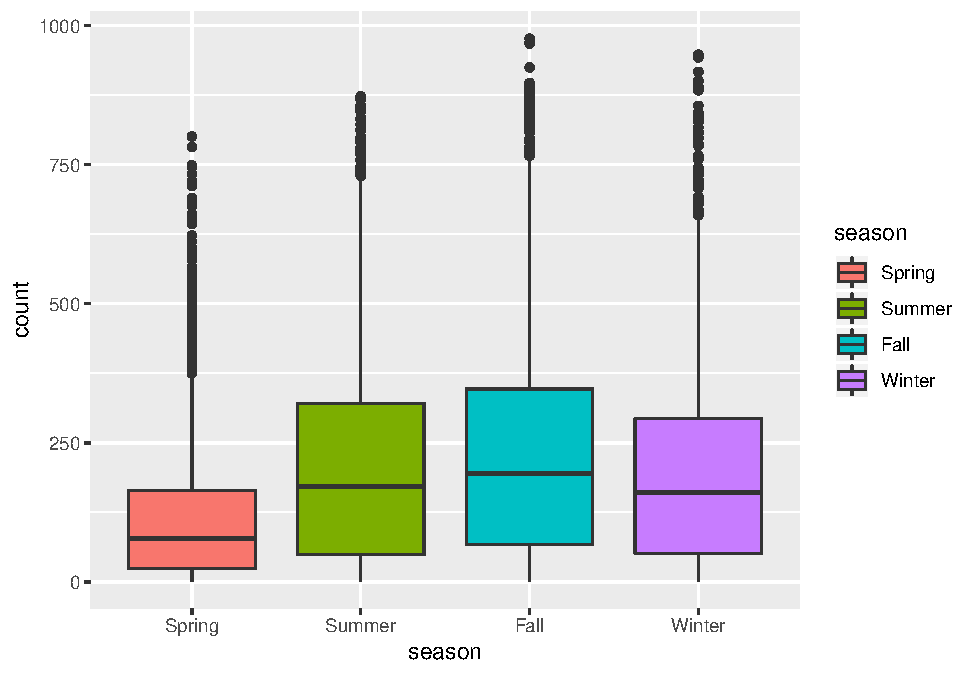
\includegraphics{BikeSharingDemand_files/figure-latex/train.mod.1.season-1.pdf}

\newpage

\hypertarget{holiday}{%
\paragraph{Holiday}\label{holiday}}

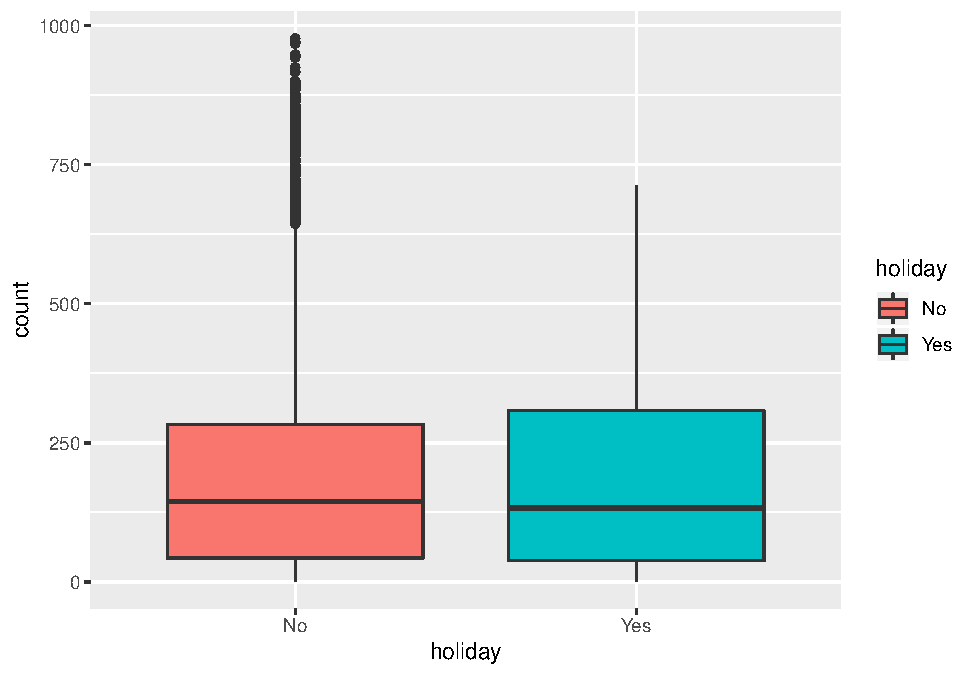
\includegraphics{BikeSharingDemand_files/figure-latex/train.mod.1.holiday-1.pdf}

\hypertarget{working-day}{%
\subsubsection{Working Day}\label{working-day}}

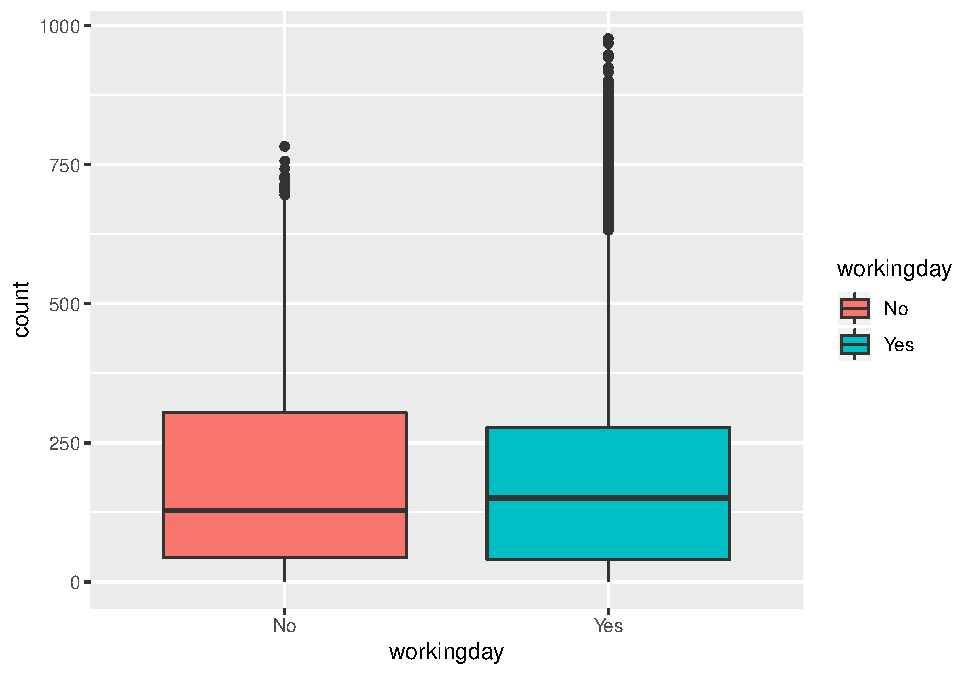
\includegraphics{BikeSharingDemand_files/figure-latex/train.mod.1.workingday-1.pdf}

\newpage

\hypertarget{weather}{%
\subsubsection{Weather}\label{weather}}

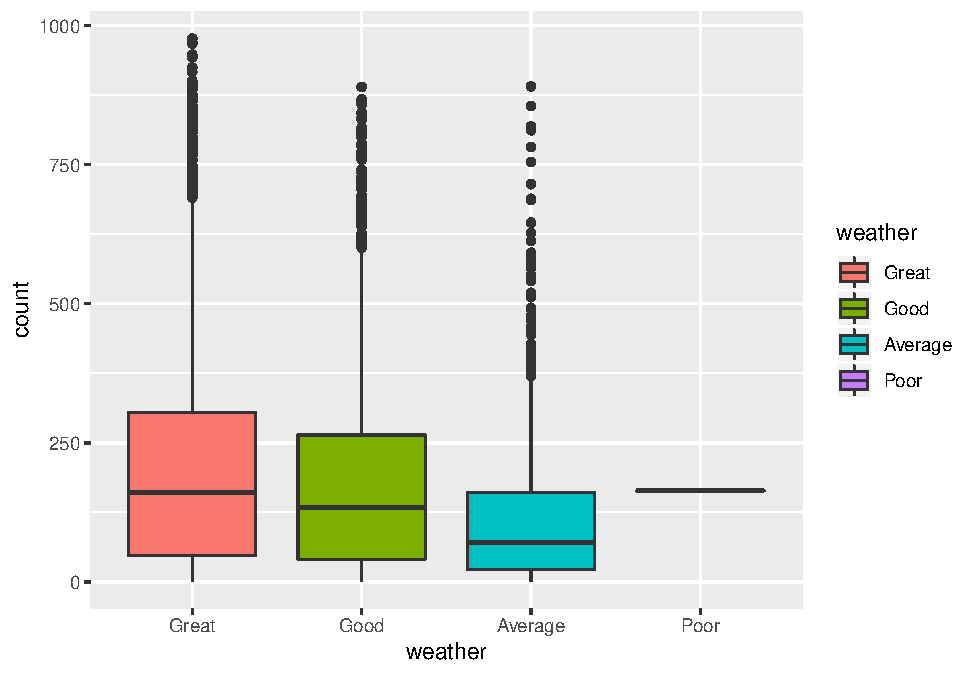
\includegraphics{BikeSharingDemand_files/figure-latex/train.mod.1.weather-1.pdf}

The datetime column was broken out into multiple factors as well so that we could visualize the components of each date and aggregate by different dimensions of the timestamp. We felt this was also necessary due to the nature of how the train/ test data sets had been pre-split. (i.e\ldots{}with the first 19 days of the month holding the only true counts to validate our models against.)

\begin{itemize}
\tightlist
\item
  Year
\item
  Month
\item
  Day
\item
  Hour
\end{itemize}

\hypertarget{month}{%
\subsubsection{Month}\label{month}}

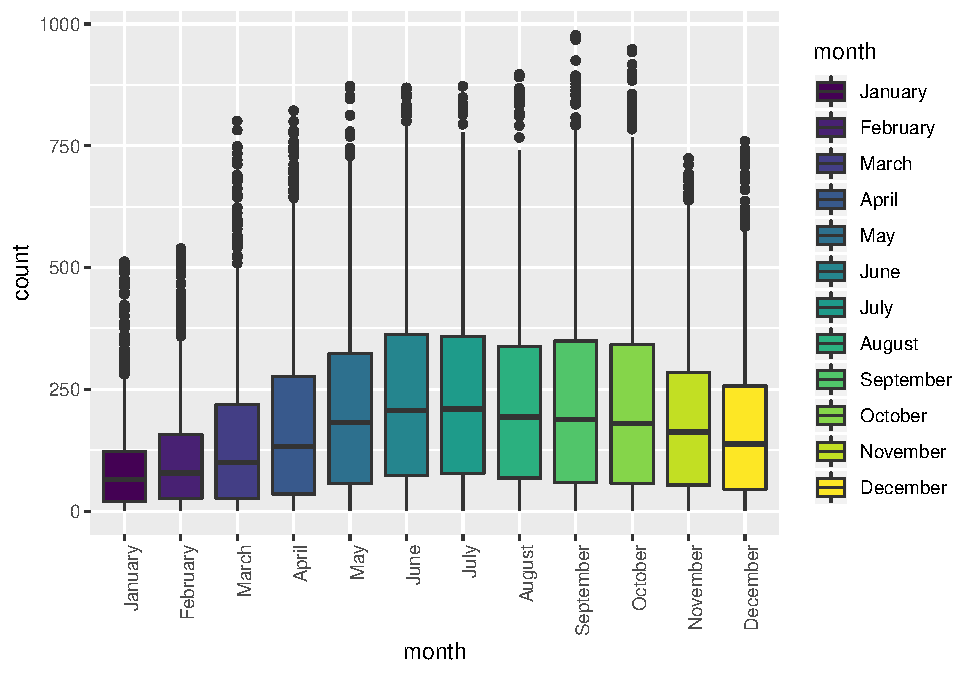
\includegraphics{BikeSharingDemand_files/figure-latex/train.mod.1.month-1.pdf}

\newpage

\hypertarget{continuous-variables}{%
\subsection{Continuous Variables}\label{continuous-variables}}

\hypertarget{count-by-temperature}{%
\subsubsection{Count by Temperature}\label{count-by-temperature}}

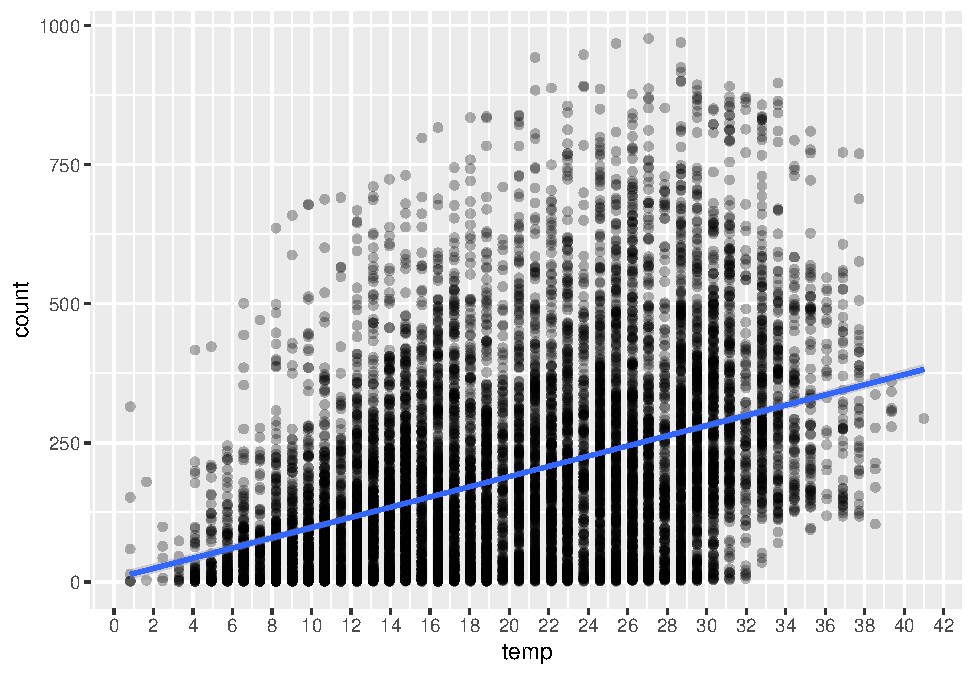
\includegraphics{BikeSharingDemand_files/figure-latex/train.mod.1.temp-1.pdf}

\newpage

\hypertarget{count-by-feels-like-temperature}{%
\subsubsection{Count by ``Feels like'' Temperature}\label{count-by-feels-like-temperature}}

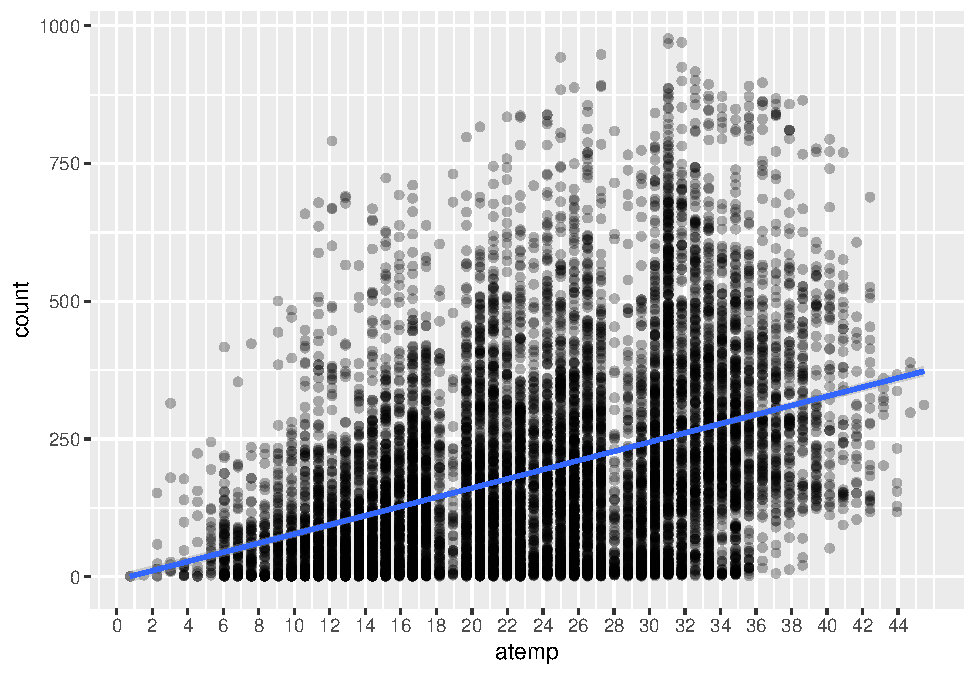
\includegraphics{BikeSharingDemand_files/figure-latex/train.mod.1.atemp-1.pdf}

\newpage

\hypertarget{count-by-wind-speed}{%
\subsubsection{Count by Wind Speed}\label{count-by-wind-speed}}

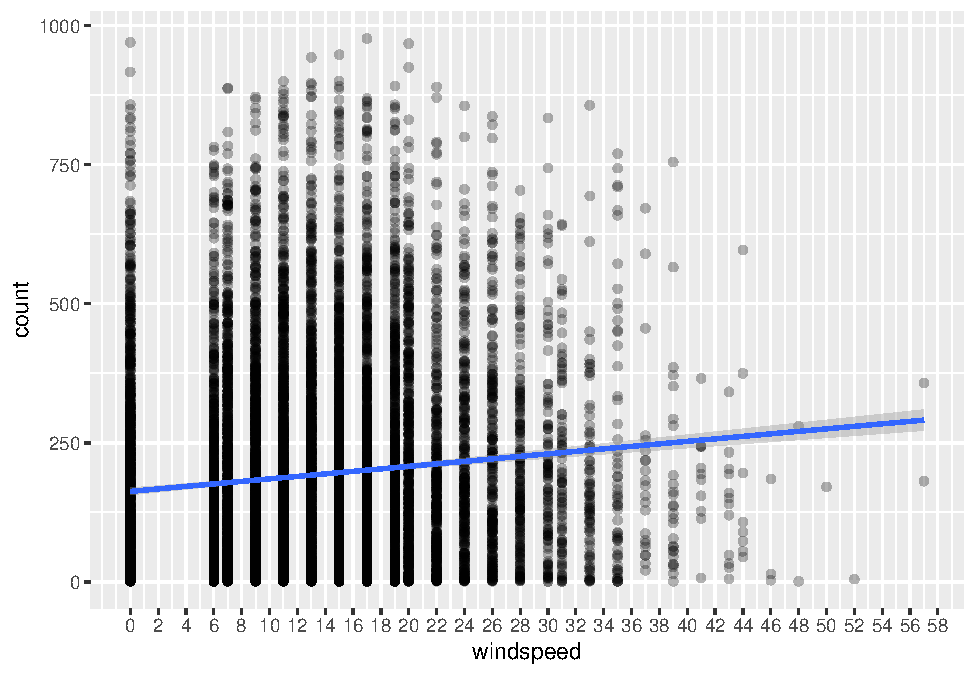
\includegraphics{BikeSharingDemand_files/figure-latex/train.mod.1.windspeed-1.pdf}

\newpage

\hypertarget{correlation-matrix}{%
\subsection{Correlation Matrix}\label{correlation-matrix}}

There are several variables with a relatively high level of covariance from the training set. The following columns should therefore be removed so as not to be picked up by any automated modelling techniques.

\begin{itemize}
\tightlist
\item
  atemp
\item
  causual
\item
  registered
\end{itemize}

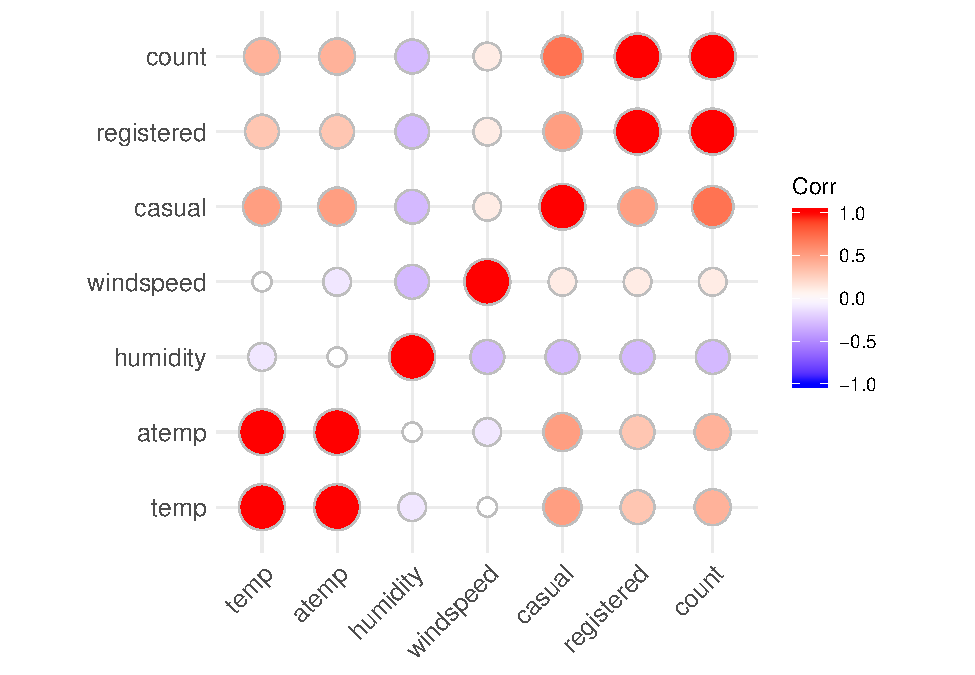
\includegraphics{BikeSharingDemand_files/figure-latex/train.mod.1.corr.matrix-1.pdf}

\newpage

\hypertarget{objective-i-analysis}{%
\section{Objective I Analysis}\label{objective-i-analysis}}

\hypertarget{question-of-interest}{%
\subsection{Question of Interest}\label{question-of-interest}}

The team be utilizing the multiple linear regression techniques we've learned up to this point in the program to predict the bike rental deman on a given date and time. The model will be evaluated on the Root Mean Squared Logarithmic Error, or RMSLE. As this data represents hourly data collected, there is an obvious time component associated with this particular competition. We wanted to gauge how effective mutiple linear regression would be when the assumption of indepdence is clearly violated.

\begin{verbatim}
## # A tibble: 12 x 5
##    month      mean    sd median observations
##    <ord>     <dbl> <dbl>  <dbl>        <int>
##  1 January    3.78  1.47   4.17          884
##  2 February   3.98  1.51   4.36          901
##  3 March      4.19  1.61   4.61          901
##  4 April      4.46  1.53   4.89          909
##  5 May        4.76  1.43   5.20          912
##  6 June       4.89  1.38   5.33          912
##  7 July       4.90  1.35   5.34          912
##  8 August     4.86  1.37   5.26          912
##  9 September  4.81  1.42   5.24          909
## 10 October    4.79  1.42   5.19          911
## 11 November   4.65  1.40   5.09          911
## 12 December   4.52  1.43   4.93          912
\end{verbatim}

\begin{verbatim}
## # A tibble: 1 x 12
##   datetime            season holiday workingday weather  temp atemp
##   <dttm>               <dbl>   <dbl>      <dbl>   <dbl> <dbl> <dbl>
## 1 2012-01-06 13:00:00      1       0          1       1  16.4  20.5
## # ... with 5 more variables: humidity <dbl>, windspeed <dbl>,
## #   casual <dbl>, registered <dbl>, count <dbl>
\end{verbatim}

\hypertarget{model-selection}{%
\subsection{Model Selection}\label{model-selection}}

\hypertarget{lasso}{%
\subsubsection{Lasso}\label{lasso}}

\begin{Shaded}
\begin{Highlighting}[]
\NormalTok{split.perc =}\StringTok{ }\FloatTok{.80}

\NormalTok{train.indices =}\StringTok{ }\KeywordTok{sample}\NormalTok{(}\DecValTok{1}\OperatorTok{:}\KeywordTok{dim}\NormalTok{(train.mod}\FloatTok{.1}\NormalTok{)[}\DecValTok{1}\NormalTok{],}\KeywordTok{round}\NormalTok{(split.perc }\OperatorTok{*}\StringTok{ }\KeywordTok{dim}\NormalTok{(train.mod}\FloatTok{.1}\NormalTok{)[}\DecValTok{1}\NormalTok{]))}

\NormalTok{train.mod.}\FloatTok{1.}\NormalTok{train =}\StringTok{ }\NormalTok{train.mod}\FloatTok{.1}\NormalTok{[train.indices,]}
\NormalTok{train.mod.}\FloatTok{1.}\NormalTok{test  =}\StringTok{ }\NormalTok{train.mod}\FloatTok{.1}\NormalTok{[}\OperatorTok{-}\NormalTok{train.indices,]}


\NormalTok{train.mod.}\FloatTok{1.}\NormalTok{train}\OperatorTok{$}\NormalTok{datetime <-}\StringTok{ }\OtherTok{NULL}
\NormalTok{train.mod.}\FloatTok{1.}\NormalTok{test}\OperatorTok{$}\NormalTok{datetime <-}\StringTok{ }\OtherTok{NULL}


\NormalTok{train.mod.}\FloatTok{1.}\NormalTok{train}
\end{Highlighting}
\end{Shaded}

\begin{verbatim}
## # A tibble: 8,624 x 12
##    season holiday workingday weather  temp humidity windspeed count year 
##    <fct>  <fct>   <fct>      <fct>   <dbl>    <dbl>     <dbl> <dbl> <fct>
##  1 Fall   No      Yes        Average 28.7        89     13.0   1.61 2012 
##  2 Spring No      Yes        Great   21.3        27     31.0   4.77 2011 
##  3 Fall   No      No         Great   28.7        54     11.0   6.17 2012 
##  4 Winter No      Yes        Great    9.84       75      0     2.30 2011 
##  5 Spring No      Yes        Good     8.2        34     19.0   4.16 2011 
##  6 Summer No      No         Good    28.7        48      6.00  5.48 2011 
##  7 Winter No      Yes        Great   13.9        46     15.0   6.30 2012 
##  8 Spring No      Yes        Great    9.02       51     20.0   4.04 2011 
##  9 Fall   No      Yes        Great   20.5        82      0     5.27 2012 
## 10 Fall   No      Yes        Great   30.3        70     19.0   5.19 2012 
## # ... with 8,614 more rows, and 3 more variables: month <ord>, day <fct>,
## #   hour <fct>
\end{verbatim}

\begin{Shaded}
\begin{Highlighting}[]
\NormalTok{x <-}\StringTok{ }\KeywordTok{model.matrix}\NormalTok{(count}\OperatorTok{~}\NormalTok{.,train.mod.}\FloatTok{1.}\NormalTok{train)[,}\OperatorTok{-}\DecValTok{7}\NormalTok{]}
\NormalTok{y <-}\StringTok{ }\NormalTok{train.mod.}\FloatTok{1.}\NormalTok{train}\OperatorTok{$}\NormalTok{count}

\NormalTok{grid=}\DecValTok{10}\OperatorTok{^}\KeywordTok{seq}\NormalTok{(}\DecValTok{10}\NormalTok{,}\OperatorTok{-}\DecValTok{2}\NormalTok{, }\DataTypeTok{length =}\DecValTok{100}\NormalTok{)}
\NormalTok{lasso.model <-}\StringTok{ }\KeywordTok{glmnet}\NormalTok{(x,y,}\DataTypeTok{alpha=}\DecValTok{1}\NormalTok{, }\DataTypeTok{lambda=}\NormalTok{grid)}

\NormalTok{xtest<-}\KeywordTok{model.matrix}\NormalTok{(count}\OperatorTok{~}\NormalTok{.,train.mod.}\FloatTok{1.}\NormalTok{test)[,}\OperatorTok{-}\DecValTok{7}\NormalTok{]}
\NormalTok{ytest <-}\StringTok{ }\NormalTok{train.mod.}\FloatTok{1.}\NormalTok{test}\OperatorTok{$}\NormalTok{count}


\NormalTok{cv.out=}\KeywordTok{cv.glmnet}\NormalTok{(x,y,}\DataTypeTok{alpha=}\DecValTok{1}\NormalTok{) }\CommentTok{#alpha=1 performs LASSO}
\KeywordTok{plot}\NormalTok{(cv.out)}
\end{Highlighting}
\end{Shaded}

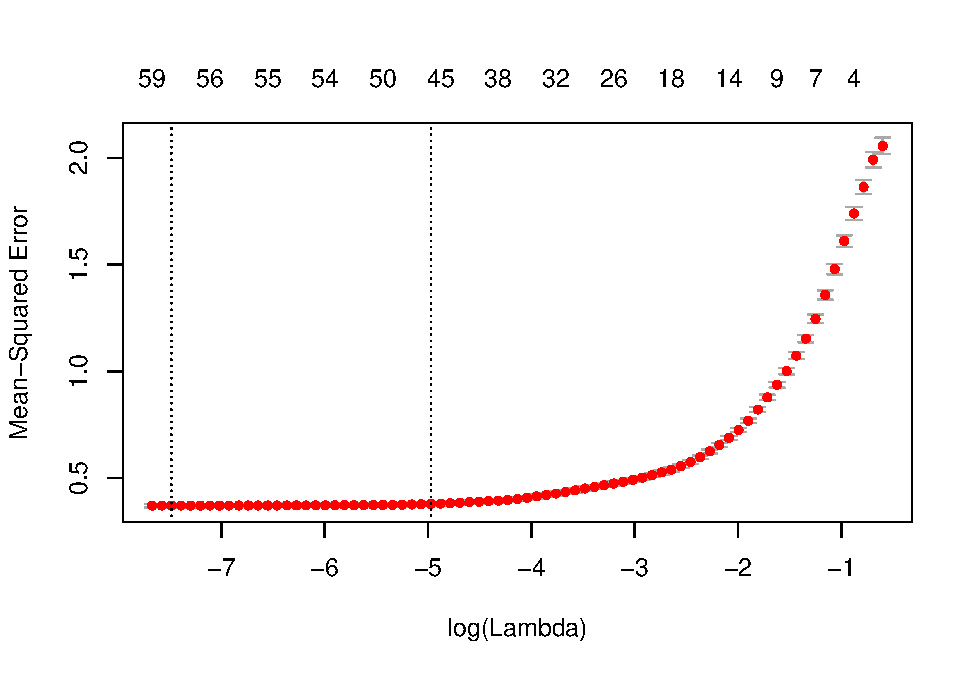
\includegraphics{BikeSharingDemand_files/figure-latex/unnamed-chunk-1-1.pdf}

\begin{Shaded}
\begin{Highlighting}[]
\NormalTok{best.lambda <-cv.out}\OperatorTok{$}\NormalTok{lambda.min  }\CommentTok{#Optimal penalty parameter.  You can make this call visually.}
\NormalTok{lasso.pred=}\KeywordTok{predict}\NormalTok{(lasso.model ,}\DataTypeTok{s=}\NormalTok{best.lambda ,}\DataTypeTok{newx=}\NormalTok{xtest)}

\NormalTok{testMSE_LASSO<-}\KeywordTok{mean}\NormalTok{((ytest}\OperatorTok{-}\NormalTok{lasso.pred)}\OperatorTok{^}\DecValTok{2}\NormalTok{)}
\NormalTok{testMSE_LASSO}
\end{Highlighting}
\end{Shaded}

\begin{verbatim}
## [1] 0.3535176
\end{verbatim}

\hypertarget{custom-variable-selection}{%
\subsubsection{Custom Variable Selection}\label{custom-variable-selection}}

We developed the best fitting model with a custom selection of variables after having accounted for those with high correlation and adding interactive terms such as month/ hour based on the seasonal nature that the box plots exhibited.

\begin{verbatim}
## Warning: not plotting observations with leverage one:
##   5555

## Warning: not plotting observations with leverage one:
##   5555
\end{verbatim}

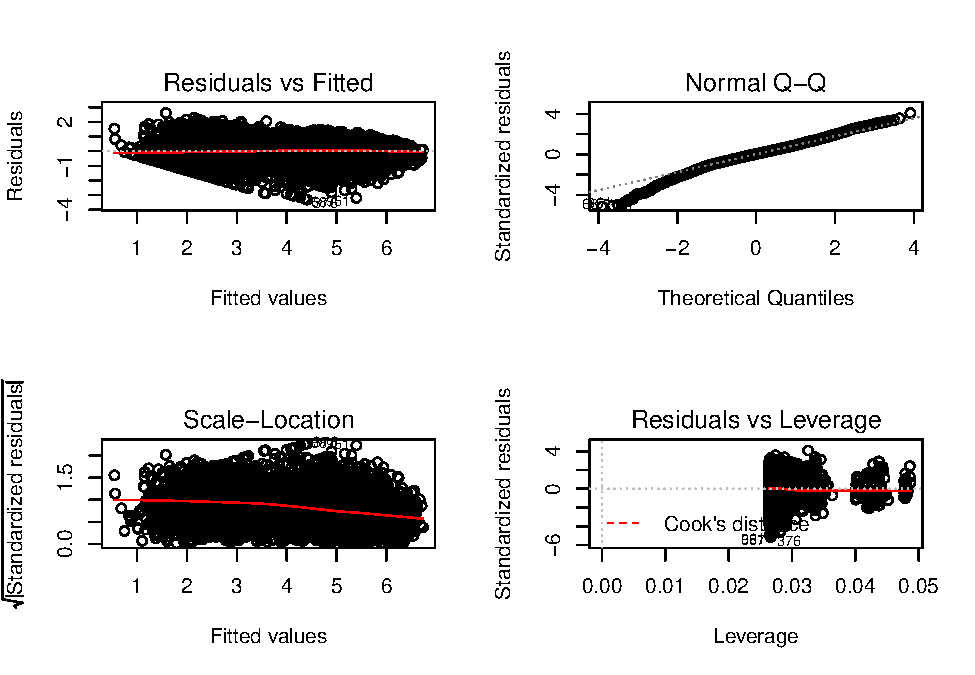
\includegraphics{BikeSharingDemand_files/figure-latex/custom-model-1.pdf} 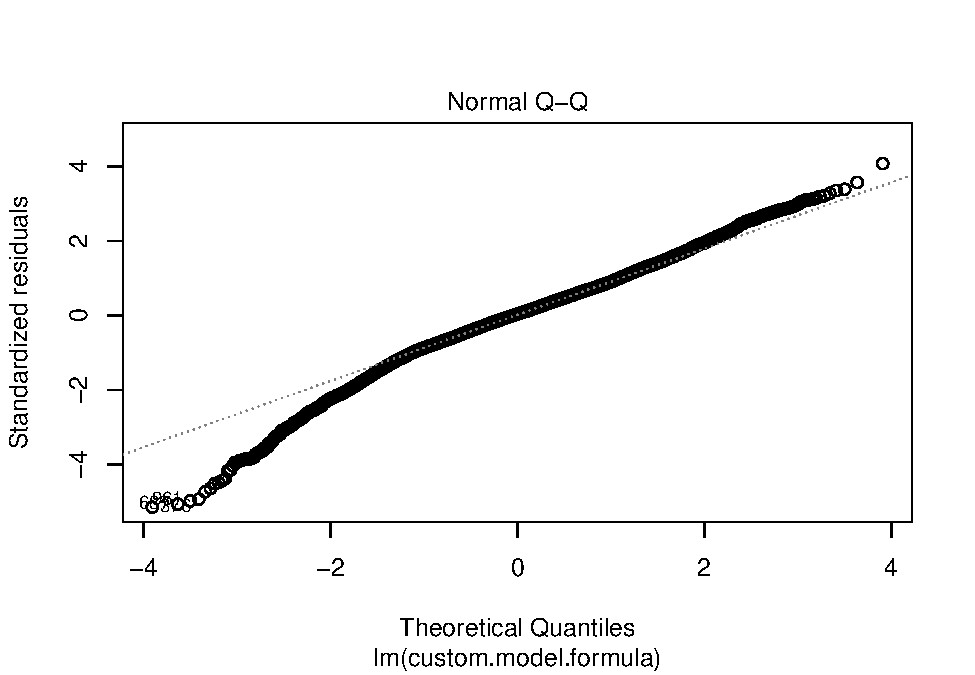
\includegraphics{BikeSharingDemand_files/figure-latex/custom-model-2.pdf}

\hypertarget{rmsle-root-mean-squared-logarithmic-error-loss}{%
\subsubsection{RMSLE: Root Mean Squared Logarithmic Error Loss}\label{rmsle-root-mean-squared-logarithmic-error-loss}}

\begin{verbatim}
## [1] 0.1923972
\end{verbatim}

\hypertarget{stepwise}{%
\subsubsection{Stepwise}\label{stepwise}}

\begin{verbatim}
## # A tibble: 6 x 10
##   datetime            season holiday workingday weather  temp atemp
##   <dttm>               <dbl>   <dbl>      <dbl>   <dbl> <dbl> <dbl>
## 1 2011-01-20 00:00:00      1       0          1       1 10.7   11.4
## 2 2011-01-20 01:00:00      1       0          1       1 10.7   13.6
## 3 2011-01-20 02:00:00      1       0          1       1 10.7   13.6
## 4 2011-01-20 03:00:00      1       0          1       1 10.7   12.9
## 5 2011-01-20 04:00:00      1       0          1       1 10.7   12.9
## 6 2011-01-20 05:00:00      1       0          1       1  9.84  11.4
## # ... with 3 more variables: humidity <dbl>, windspeed <dbl>, count <dbl>
\end{verbatim}

\newpage

\hypertarget{model-assumptions-assessment}{%
\subsection{Model Assumptions Assessment}\label{model-assumptions-assessment}}

\begin{itemize}
\tightlist
\item
  The response variable is linear
\item
  The data is normally distributed
\item
  Independence
\end{itemize}

\hypertarget{comparing-competing-models}{%
\subsection{Comparing Competing Models}\label{comparing-competing-models}}

\newpage

\hypertarget{parameters}{%
\subsection{Parameters}\label{parameters}}

\protect\hyperlink{parameters}{Parameters}

\hypertarget{model-interpretation}{%
\subsection{Model Interpretation}\label{model-interpretation}}

\protect\hyperlink{model-interpretation}{Model Interpretation}

\hypertarget{conclusion}{%
\subsection{Conclusion}\label{conclusion}}

\protect\hyperlink{conclusion-1}{Conclusion}

\newpage

\hypertarget{objective-ii-analysis}{%
\section{Objective II Analysis}\label{objective-ii-analysis}}

\hypertarget{question-of-interest-1}{%
\subsection{Question of Interest}\label{question-of-interest-1}}

{[}Discuss time series method{]}

\textbf{Time-Series Analysis}

{[}Details goe here{]}

\hypertarget{model-assumption-assessment}{%
\subsection{Model Assumption Assessment}\label{model-assumption-assessment}}

\protect\hyperlink{model-assumption-assessment}{Model Assumption Assessment}

\hypertarget{comparing-competing-models-1}{%
\subsection{Comparing Competing Models}\label{comparing-competing-models-1}}

\hypertarget{conclusion-1}{%
\subsection{Conclusion}\label{conclusion-1}}

\protect\hyperlink{conclusion-1}{Conclusion}

\newpage

\hypertarget{appendix}{%
\section{Appendix}\label{appendix}}

\hypertarget{code}{%
\subsection{Code}\label{code}}

\newpage

\renewcommand\refname{References}
\bibliography{references.bib}


\end{document}
